\chapter{Properties of an n-channel enhancement MOSFET}


\section{Objectives}
\begin{itemize}
    \item To find the voltage-current characteristics of a n-channel enhancement MOSFET
    \item To evaluate different operation modes of a n-channel enhancement MOSFET
\end{itemize}

\section{Materials}
\begin{itemize}
    \item Breadboard
    \item Capacitors
    \item DC power supply
    \item Digital Multi-Meter
    \item \hyperref[2N7000_1]{MOSFET (2N7000)}
    \item Resistors
\end{itemize}

\section{Introduction}
    \subsection{Circuit Diagram}
    \begin{figure}[h]
        \centering
        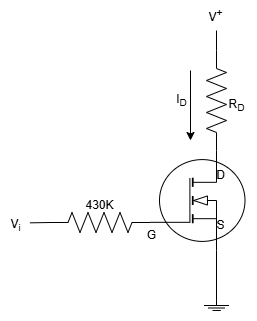
\includegraphics[width=0.65\linewidth]{Lab08/Lab8.drawio.png}
        \caption{Circuit Diagram}
        \label{l8f}
    \end{figure}
    \FloatBarrier
In Fig.\ref{l8f}, $V^+=12V$, $R_D=470\Omega$, $V_{TN}=1.40V$, $K_n=80A/V^2$.
\section{Detailed Procedures}
    \subsection{Analyzation}
    First, we find the relationship between $V_i$ and $V_{DS}$:
    \begin{equation}
        \begin{cases}
            12-R_DK_n(V_i-1.4)^2=V_{DS} & V_i>1.4\\
            \frac{12}{1+R_DK_n+2R_DK_n(V_i-1.4)}=V_{DS} & V_i\le1.4\\
        \end{cases}
    \end{equation}

    \subsection{Procedures}
    
    
\section{Discussion}


\section{Conclusion}
